\chapter{Strukturbestimmung und reziprokes Gitter}


Beugungs- und Streuexperimente, Experimente werden mit verschiedenen Teilchen
durchgeführt (Photonen, Neutroonen, Neutronen, Elektronen \(\rightarrow\) als
Wellen)

pic4

Amplitude: \(A(t)=A_0e^{-i(\omega_0t-\vec k_0\vec r)}\)
Amplitude der gestr. Welle: \( A_z(t)=\frac {A'} R e^{-i(\omega_0t-kR)}\)
Phasendifferenz: \(\left. \Delta\phi \right|_{|\vec k|=|\vec k_0|}=\Delta
s k= (\vec k - \vec k_0)\vec r\)
Elastische Streuung!; die Welle ist nur 1x gestreut \(\rightarrow\) Bornsche
Näherung

Volumen Element \(dV\) am Ort \(\vec r\):

\[dA_s(\vec r,t)=\rho(\vec r)A_z(t)dV=\frac {A'}{R_1}\rho(\vec
r)e^{-i(\omega_0t-kR_1+(\vec k-\vec k_0)\vec r)}dV\] 

\(\rho(\vec r)\)-Streudichteverteilung \(R_1\approx R_0\)

\[A_s(\vec r,t)=\frac {A}{R_0}e^{-i(\omega_0t-kR_0)}A(\vec k-\vec k_0)\]

Streuamplitude A mit dem Streuvektor (k-k0)

\[A(\vec k - \vec {k_0}) = \int_V \rho(\vec r) e^{-i(\vec k -\vec {k_0})\vec r}dV\]

\(A(\vec Q)\) ist die Fourier-transformierte \(\rho(\vec r)\);

Strukturbestimmung:
\[\rho(\vec r) = \frac 1 {(2\pi)^3}\int_{Q-Raum}A(\vec Q) e^{i\vec Q \vec r}
d^3Q\]

\section{Reziprokes Gitter}

\(\vec A\) Gitter;  \(\vec B\) reziprokes--Gitter; \(b_i:=\) Basisvektor der blz.  Raums 

\(\vec A= m_1\vec a_1+m_2\vec a_2 + m_3\vec a_3 \Rightarrow \vec B = n_1\vec b_1+n_2\vec b_2 + n_3\vec b_3 \)

\[\vec b_1 = 2\pi \frac{\vec a_2 x \vec a_3}{\vec a_1(\vec a_2 x \vec a_3}=2\pi
\frac{\vec a_2 x \vec a_3}{V_z}\]

\(V_z\) das Volumen der Elementarzelle des realen Gitters.

\[\vec b_2= 2\pi\frac{\vec a_3 x \vec a_1}{V_z}\]
\[\vec b_3= 2\pi\frac{\vec a_1 x \vec a_2}{V_z}\]
\[\vec b_1(\vec b_2 x \vec b_3)=\frac {(2\pi)^3}{V_z}; V_B=\frac
{(2\pi)^3}{V_A}\]

für rechtwinklige Krinstallsysteme: 
\[\vec b_{1,2,3}=\frac {2\pi}{a^2_{1,2,3}}\vec a^2_{1,2,3}; |\vec b_1=
\frac{2\pi}{|\vec a_1|}\]

Eigenschaften: 

\begin{itemize}
\item \(\vec a_i\vec b_i=2\pi\sigma_{ij}\)
\item reziprokes Gitter für reziprokes Gitter ist reale Gitter
\item \(V_b=\frac {(2\pi)^3}{V_a}\)
\item \(\vec A\cdot\vec B = 2\pi n\) mit \(n\in \mathbb N\) \(\rightarrow e^{\vec A\cdot\vec B }=1\)
\end{itemize}

Theorem: \(\vec B \rightarrow Kristallebenen  \perp \vec B\) und mit Abstand \(d\)


\section{Millersche Indizes}
William Miller (1839)

Millersche Indizes dienen der eindeutigen Bezeichnung von Ebenen und Richtungen
(Vektoren) in Kristallsystemen. Nach Definition: 3 ganszählige Indizes
\((h,k,l)\). Diese Indizies bezeichnen verschiedene Ebenen. Die Ebene, die durch
drei Punkte geht:

\[ \frac 1 h\vec a_1, \frac 1 k\vec a_2, \frac 1 l\vec a_3\]

pic 1 TODO

Basisvektoren schneiden die Ebenen \((h,k,l)\) gerade an den Kehrwerten \(\frac 1
h, \frac 1 k,  \frac 1 l\)

z.B. für kubisches Gitter

\[\{100\}=\begin{cases} 
(100)\\
(\overline 1 00)\\
(010)\\
(0\overline 1 0)\\
(001)\\
(00\overline 1)\\
\end{cases} 
\]
Gitttervektoren \([u,v,w]\) nur(!) im Kubischen Kristall:: Vektor
\(\underbrace{[u,v,w]}_{u\vec a_1+v\vec a_a+w\vec a_3+} \perp
\text{Ebene}(u,v,w)\); \([1,0,0]\) Würfelkante; \([110]\) Flächendiagonale; \([111]\) Raumdiagonale


\section{Brillouin-Zone}

Die Brillouin Zone ist eine Elementarzelle des reziproken Gitters. 

1.BZ \(\stackrel{\mathrm{def}}=\) die Wigner-Seitz-Zelle des reziproken Gitters

pic 2 TODO 

\[
\begin{array}{cc} reelle Gitter (Ortsraum)&reziprokes Gitter (Impulsraum)\\
sc&sc\\
bcc&fcc\\
fcc&bcc
\end{array}
\]



\section{Beugung an Periodischen Strukturen}

pic 3 TODO

Streuamplitude: 
\[A(\vec k -\vec k')=A(\vec Q)=\int_{V_0\leftarrow\text{Probevolumen}}e^{-i(\vec  Q\vec r) d^3r}\]

\[ A(\vec Q) = \underbrace{\sum_{\text{alle EZ}}e^{-i(\vec  Q\vec r)}\cdot}_{\text{Gitterfaktor}} \sum_{\text{alle
    Atome}\alpha}e^{-i(\vec  Q\vec r_\alpha)}\cdot \underbrace{\int_{\text{Atom }\alpha}
\rho_\alpha(\vec r')\cdot e^{-i(\vec  Q\vec
  r')d^3r'}}_{f'_\alpha\text{-Atomstreufaktor (spez. für Atom)}}\]



note todo: zweite Summe und Integrall: underbrace (Strukturfaktor)

Braggsche Beugungsbedingung:

pic 4 TODO

\[ 2dsin\theta=n\lambda\]


\section{Streubedingung}

Für die Streuintensität :

 \[I(Q) \propto | A(\vec
Q)|^2=|\int_{V_p}\rho(\vec r) e^{-i\vec Q\vec r}|^2\]

mit \(\vec Q = \vec k - \vec k_0\)

Entwicklung von \(\rho(\vec r)\) in eine 3D Fouurier - Reihe:

\[ \vec G_{hkl} = h\vec b_1+ k\vec b_2+ l\vec b_3 \]

\(\vec b_i\) sind Basisvektoren des reziproken Gitters \(G\)

\[ \rho (\vec r) = \sum_{hkl} \rho_{hkl}e^{i\vec G_{hkl}\vec r} \]

Mit Fourier-Koeffizienten

\[ \rho_{hkl} = \frac 1 {V_z}\int_{V_z}\rho_z e^{-\vec G_{hkl}\vec
  r}dV \]

\[ \rho(\vec r) = \rho (\vec r+\vec R)\]
\[ R=m_1\vec a_1+m_2\vec a_2+m_3\vec a_3\]

\(V_z\) - Volumes des primitiven E.Z.

\[ e^{-\vec G_{hkl}\vec r}=  e^{-\vec G_{hkl}(\vec r+\vec R} \]
\[ e^{-\vec G_{hkl}\vec r}=1, \vec G_{hkl}\vec R= 2\pi N, \text{mit N
  eine ganze Zahl} \]

\[\vec a_i \vec b_i = 2\pi \sigma_{ij};  \vec G_{hkl} = \vec G = \vec
B = n_1 \vec b_1 +  n_2 \vec b_2 + n_3 \vec b_3; n_1=h, n_2=k; n_3=l; \]

\[  | A(\vec Q)|^2= |\sum_{hkl}\rho_{hkl}\int_{V_p} e^{-i(\vec B-\vec
  Q)\vec r} dV|^2 \]

\[ 
\int_{V_p} e^{-i(\vec B-\vec Q)\vec r} dV = =\begin{cases}
  V_p,  & \text{für } \vec Q=\vec B \\
  0, & \text{für } \vec Q\neq\vec B
\end{cases}
\]

(Laue) Streubedingung: \(\vec k - \vec k_0 = \vec Q= \vec B \)
z.B Braggsche Streubedingung

 
%\includegraphics[width=0.75\textwidth]{06_01.png}
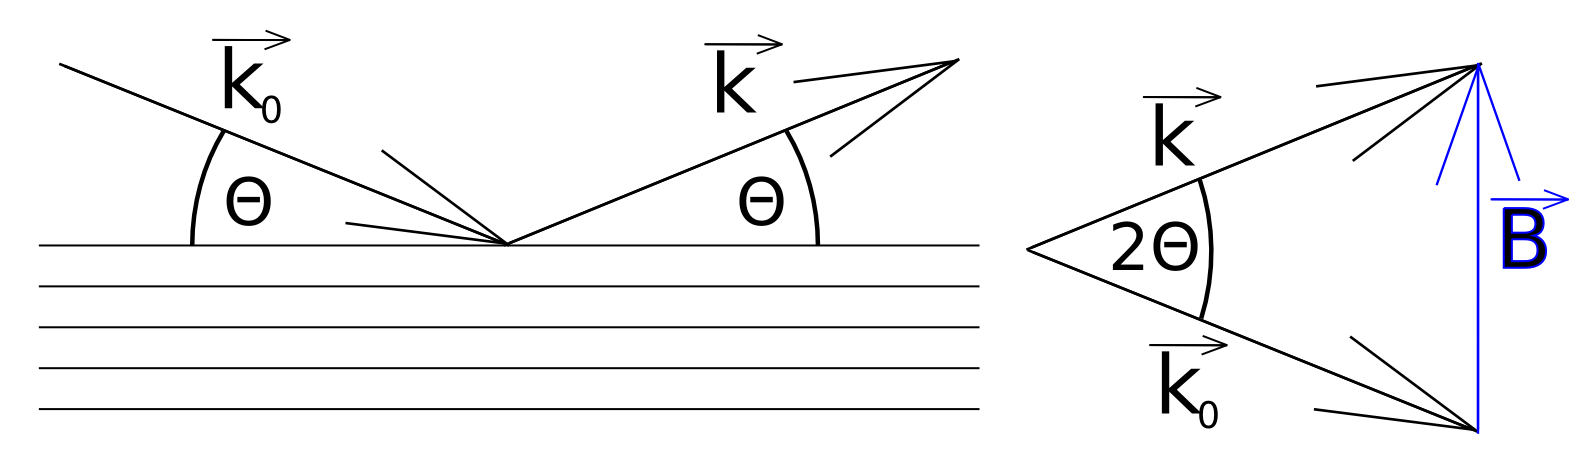
\includegraphics[width=0.75\textwidth]{kap03_03.png}

\[ d = d_{hkl} = \frac {2\pi}{|\vec B|}\]
\[|\vec B| =  \frac {2\pi}{d} =2
\frac {2\pi}{\lambda}2sin\theta \]

\[ n\lambda = 2dsin\theta, \lambda << d\]

\section{Ewald-Kugel}

%\includegraphics[width=0.75\textwidth]{06_02.png}
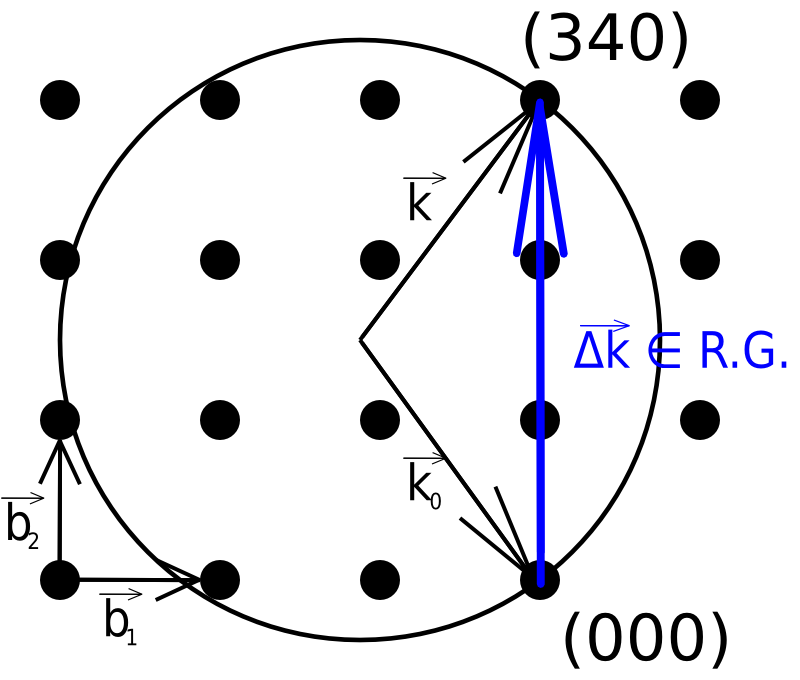
\includegraphics[width=0.75\textwidth]{kap03_04.png}


\begin{itemize}
\item zeichne die Punkte des reziprokes Gitters
\item der Wellenvektor \(\vec k_0\) endet am Punkt \((000)\)
\item der Anfangspunkt von \(\vec k_0\) ist \(M\)
\item alle Wellenvektoren mit \(|\vec k|= |\vec k_0|\) auf der
  Kugelfläche enden
\item Beugungsmaximums treten auf bei \(\vec k= \vec k_0 +\vec B\)
\end{itemize}

Die Reflexe sind ``verschmiert'' aus verschiedenen Gründen:
\begin{itemize}
\item Kristall mit englicher Abmessung
\item Defekte
\item Temperatur
\item die endliche Fequenz-Schärfe \(\Delta f\) der Strahlung
\end{itemize}

\section{Strukturfaktor}

\[  A(\vec Q)= \underbrace{\sum_{\text{aller E.Z.}}e^{-i\vec Q\vec
  R}}_{\text{Gitterfaktor}}\cdot \underbrace{\sum_{\text{aller Atome d}}e^{-i\vec Q\vec r_{\alpha}} f_{\alpha}}_{S(\vec Q) \text{Strukturfaktor}}
\]


Strukturfaktor bestimmt Intensität; Ausläschung möglich

Gittervektor: \( \vec B = n_1 \vec b_1 +  n_2 \vec b_2 + n_3 \vec b_3;
\vec r_\alpha = u_\alpha\vec a_1 + v_\alpha\vec a_2 +w_\alpha\vec a_3\)

\[ S(\vec Q) = S_{skl} = \sum_\alpha f_\alpha(\vec Q)
e^{-i\vec Q\vec r_\alpha}; \vec a_i\vec b_i=2\pi \sigma_{ij}
\]


\[  S_{hkl} = \sum_\alpha f_\alpha(\vec Q) e^{-i2\pi( h\cdot u_\alpha
  + k\cdot v_\alpha +l\cdot w_\alpha)}\]
z.B. bcc Gitter mit \(\vec r_1 = (000); \vec r_2 = (\frac 1 2, \frac 1
2, \frac 1 2); f_1=f_2\)

\[  S_{hkl} =f_1\left[1 + e^{-i\pi( h + k +l)}\right]=\begin{cases}
  2f_1,  & (h+k+l) \text{gerade } \\
  0, & (h+k+l) \text{ungerade }
\end{cases}
\]

\section{Methoden der Strukturanalyse}

\(\lambda \leq 2d; \lambda \approx 1A\)

\underline{Röntgenstralen} Quellen sind Röntgenröhre oder
Synchrotronstralung (\(e^-\) auf Kreisbahnen ANKA, KIT)



%\includegraphics[width=0.75\textwidth]{06_03.png}
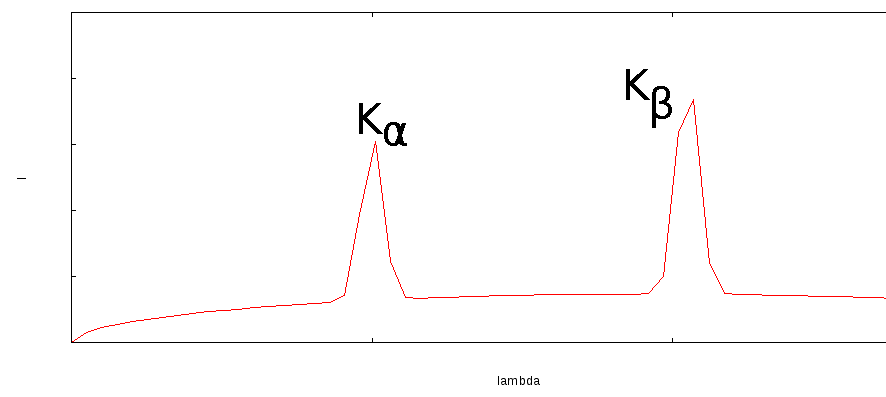
\includegraphics[width=0.75\textwidth]{kap03_05.png}



\[ E = h\nu = \frac {hc}{\lambda}, \lambda \approx 1 A, E\approx
10eV\]

1) \underline{Röntgenstrahlen}:

\begin{itemize}
\item Streuung an Elektronen
\item Formfaktor \(f_\alpha \approx Z (\text{Atomzahl}); I\approx Z^2\)
\item leichte Elemente schwer nachweisbar
\end{itemize}

2) \underline{Neutronen}  Spin \(\frac 1 2\) \(E=\frac {p^2}{2m_N}=\frac
{h^2}{2m_N\lambda^2}\approx 100meV\)

\begin{itemize}
\item Streuung an Kernen über starke Wechselwirkung (WW)
\item Elektronen in der Hülle mag. Moment tragen
\end{itemize}

Quellen: Forschungsreaktoren (Jülich, grenoble,...)

3) \underline{Elektronen} \(E=\frac {p^2}{2m_N}=\frac
{h^2}{2m_e\lambda^2}\approx 100eV\)
\begin{itemize}
\item Couulomb WW mit Elektronen und Kernen
\item sehr geringe Eindringtiefe
\item Oberflächenphysik LEED-Methode (low energy electron difraction)
\item TEM = Transmissionselektronenmikroskopie; dünne Schichten
\end{itemize}


\section{Experimentelle Beugungsverfahren}

\begin{itemize}
\item \underline{Laue-Verfahren} kontinuierliches (\(\lambda\))
  Spektrum, Einkristall

%\includegraphics[width=0.75\textwidth]{07_02.png}
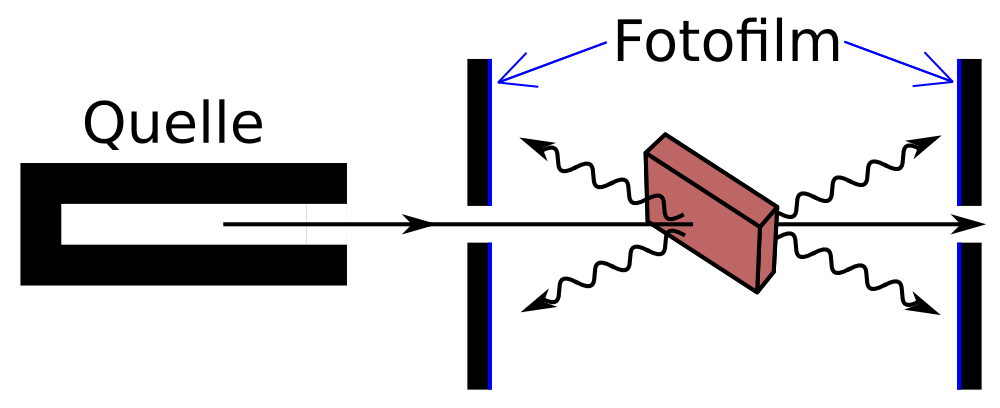
\includegraphics[width=0.75\textwidth]{kap03_06.png}


\begin{itemize}
\item Ewald-Kugel hat ``dicke Haut''
\item viele Reflexe gleichzeitig
\end{itemize}

Anwendungen:
 \begin{itemize}
 \item Orientierung der Symetrieachse
 \item Ist die Probe wirklich ein Einkristall
 \end{itemize}

\item Drehkristallvefahren: monochromatische Strahlung, und Kristall
  ist gedreht

%\includegraphics[width=0.75\textwidth]{07_03.png}
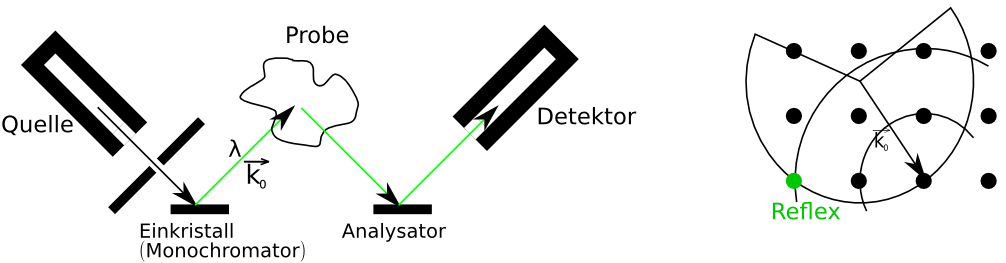
\includegraphics[width=0.75\textwidth]{kap03_07.png}

Einkristall ermöglicht die Drehung von \(\vec k_0\)

\item Debye-Scherer-Verfahren: monochromatische Strahlung

  \begin{itemize}
  \item monochromatische Strahlung
  \item Pulver oder feinkörniger Pulverkristall
  \end{itemize}


%\includegraphics[width=0.75\textwidth]{07_04.png}
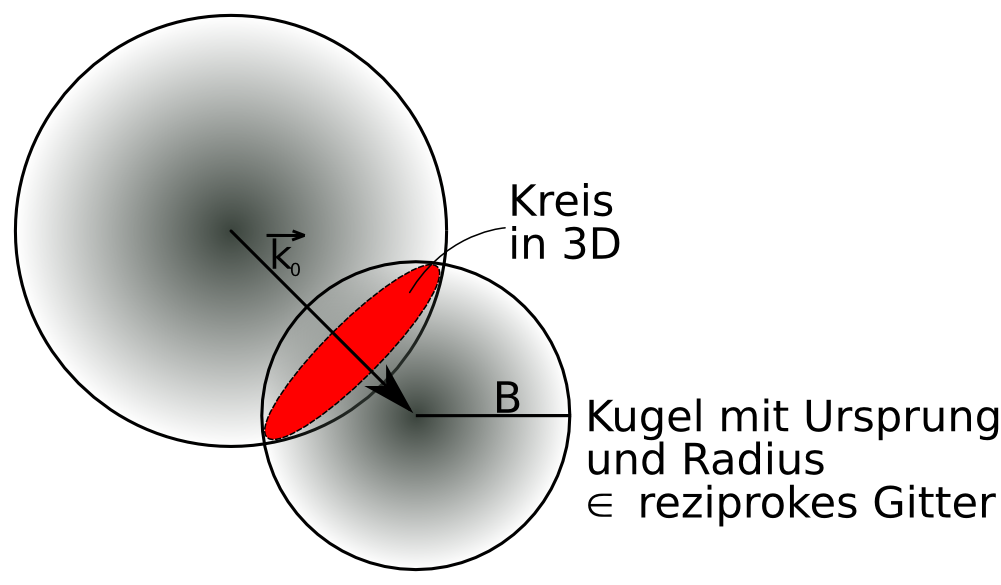
\includegraphics[width=0.75\textwidth]{kap03_08.png}

\(\vec B\) dreht um \(4\pi\) Raumwinkel \(|\vec B| \leq 2|\vec k_0|\);\(\frac{\Delta \vec k_0}{ \vec k_0}\approx 10^{-4}\)

pic 5 TODO

\begin{itemize}
\item ein bestimmer Reflex in alle Richtuungen vorhanden
\item Gitterkonstanten-Messung \(\frac {\Delta a}{a}\approx 10^{-5}\)
\end{itemize}

\end{itemize}



